\documentclass[10pt,a4paper]{article}

\usepackage[utf8]{inputenc}
\usepackage[T1]{fontenc}
\usepackage{lmodern}
\usepackage[margin=1.8cm,top=1.8cm,bottom=1.8cm]{geometry}
\usepackage{amsmath,amssymb}
\usepackage{booktabs}
\usepackage{graphicx}
\usepackage{xcolor}
\usepackage{tabularx}
\usepackage{enumitem}
\usepackage{tcolorbox}
\usepackage{caption}
\usepackage{subcaption}
\usepackage[hidelinks,colorlinks=true,linkcolor=blue!70!black,citecolor=teal!70!black,urlcolor=blue!70!black]{hyperref}
\usepackage{cleveref}

\definecolor{boxgray}{RGB}{245, 247, 250}
\definecolor{bordergray}{RGB}{210, 215, 225}

\tcbset{
    colback=boxgray,
    colframe=bordergray,
    boxrule=0.7pt,
    arc=2pt,
    left=6pt,
    right=6pt,
    top=4pt,
    bottom=4pt
}

\title{\vspace{-1.2cm}\textbf{\Large Project Scoping Document (Week 2): Vibrant Tractography Pipeline}\\[0.2em]
\textbf{\large TRX-Driven Variable Tube Thickness (Rounded Cones), Opacity, and Color}}
\author{\textbf{Team 3} (3 Students) \quad | \quad MSc Visual Computing}
\date{Academic Year 2026/2027}

\begin{document}

\maketitle

\vspace{-0.3cm}
\begin{tcolorbox}
\textbf{Project Goal:} Upgrade Vibrant's tractography renderer to ingest modern \textbf{TRX files} and drive \textbf{variable-thickness rounded cones}, \textbf{opacity}, and \textbf{color} from biological streamline attributes, eliminating the visual clutter of uniform-radius capsules.
\end{tcolorbox}

\vspace{-0.2cm}
\section{Motivation and Context}
Vibrant \cite{kraaijeveld2024voxel} is an open-source tool for 3D brain anatomy and tractography that ray-traces streamlines using a coarse voxel grid. In the current version, Vibrant only loads legacy \texttt{.tck} files and draws all streamlines as uniform capsules of fixed radius ($r = \text{const}$) and uniform opacity (\Cref{fig:current_state}). This creates dense ``spaghetti clutter'' (\Cref{fig:hero}), occluding deep brain structures and preventing visual encoding of quantitative tract properties.

\begin{figure}[ht!]
    \centering
    \begin{subfigure}[b]{0.47\textwidth}
        \centering
        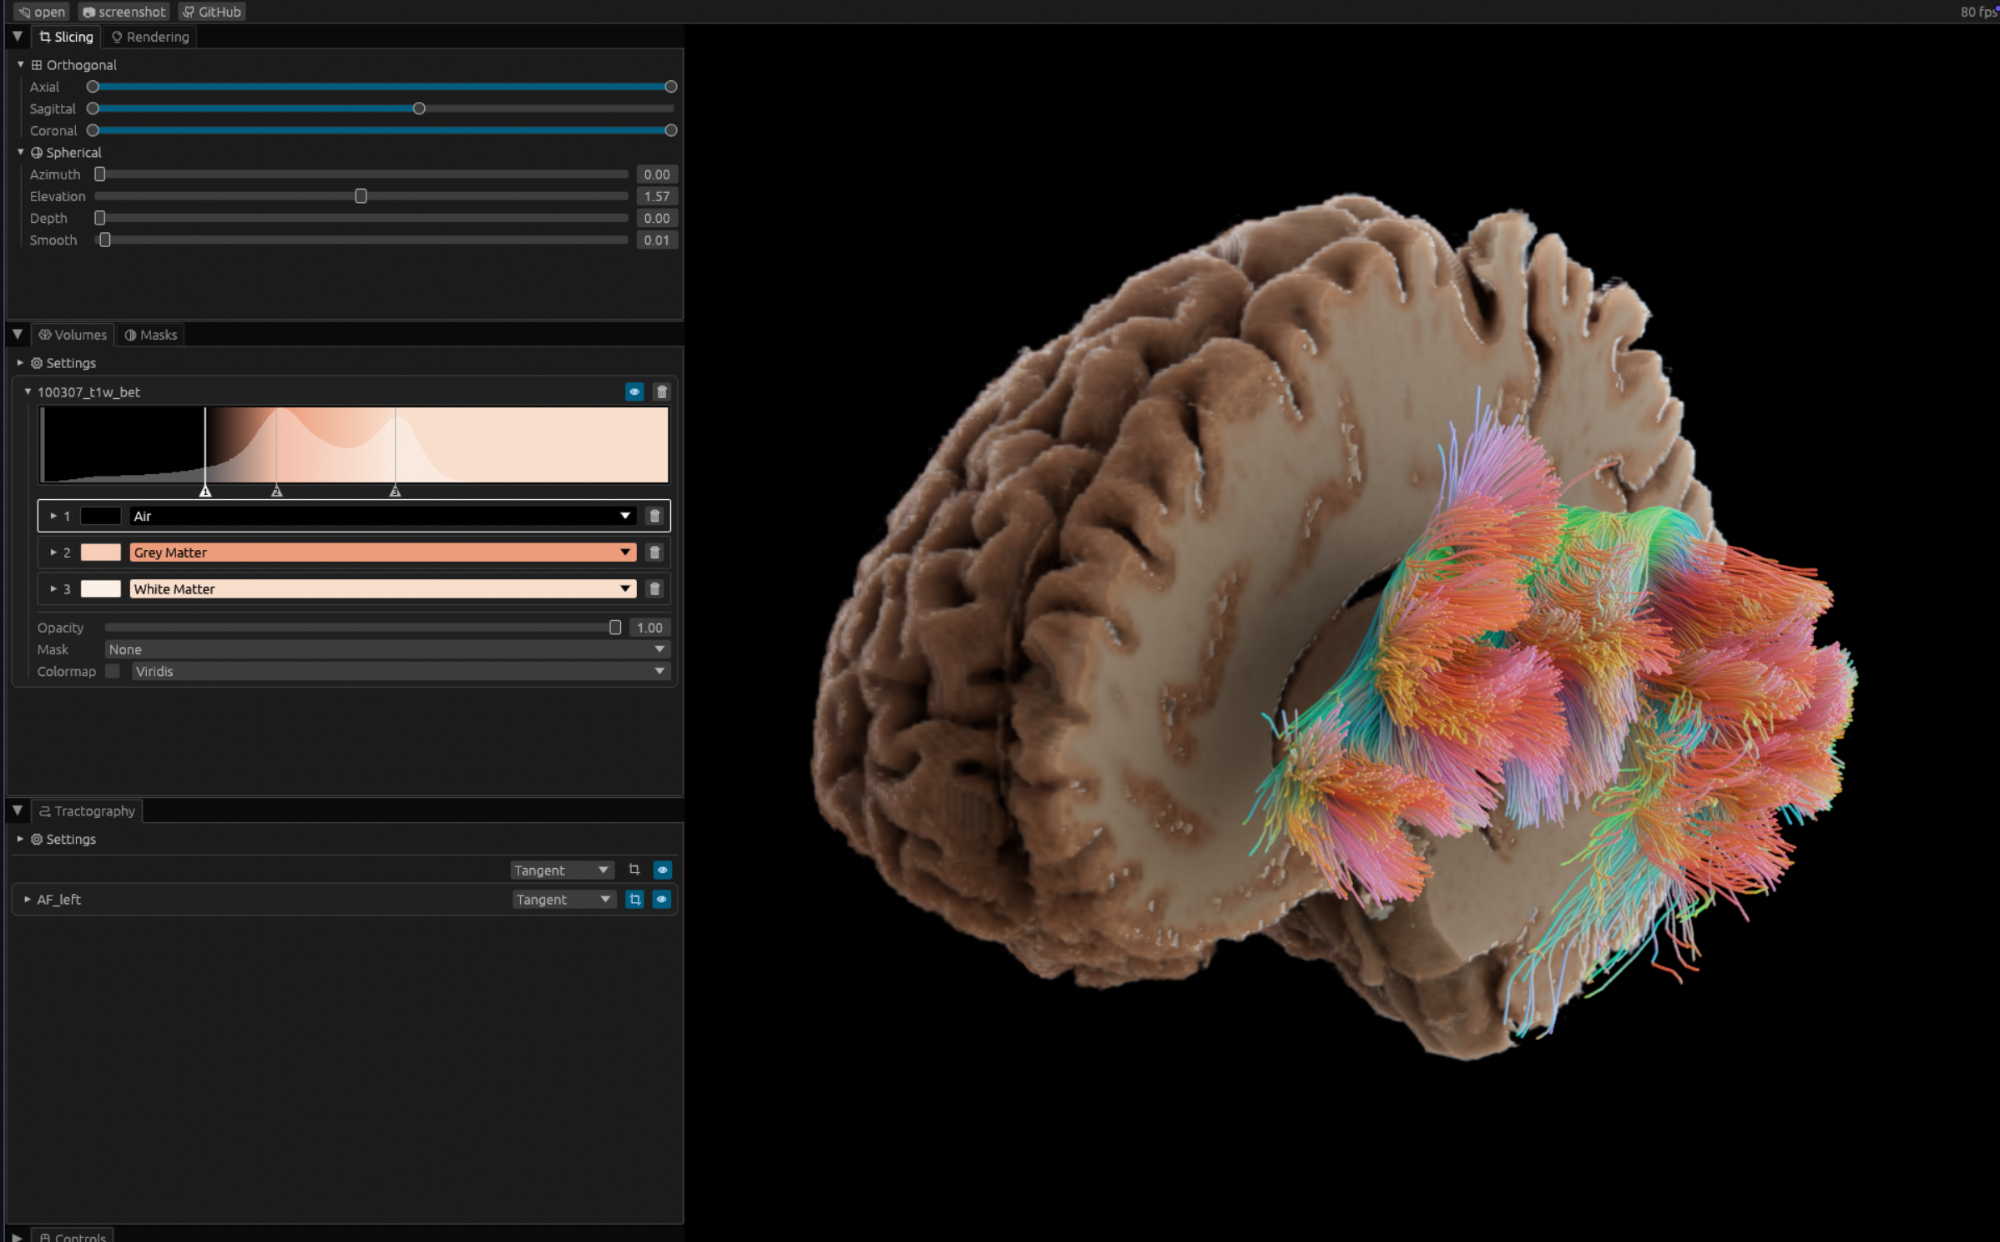
\includegraphics[width=\textwidth]{figures/vibrant-ui.png}
        \caption{Current state: Constant-radius streamline capsules.}
        \label{fig:current_state}
    \end{subfigure}
    \hfill
    \begin{subfigure}[b]{0.47\textwidth}
        \centering
        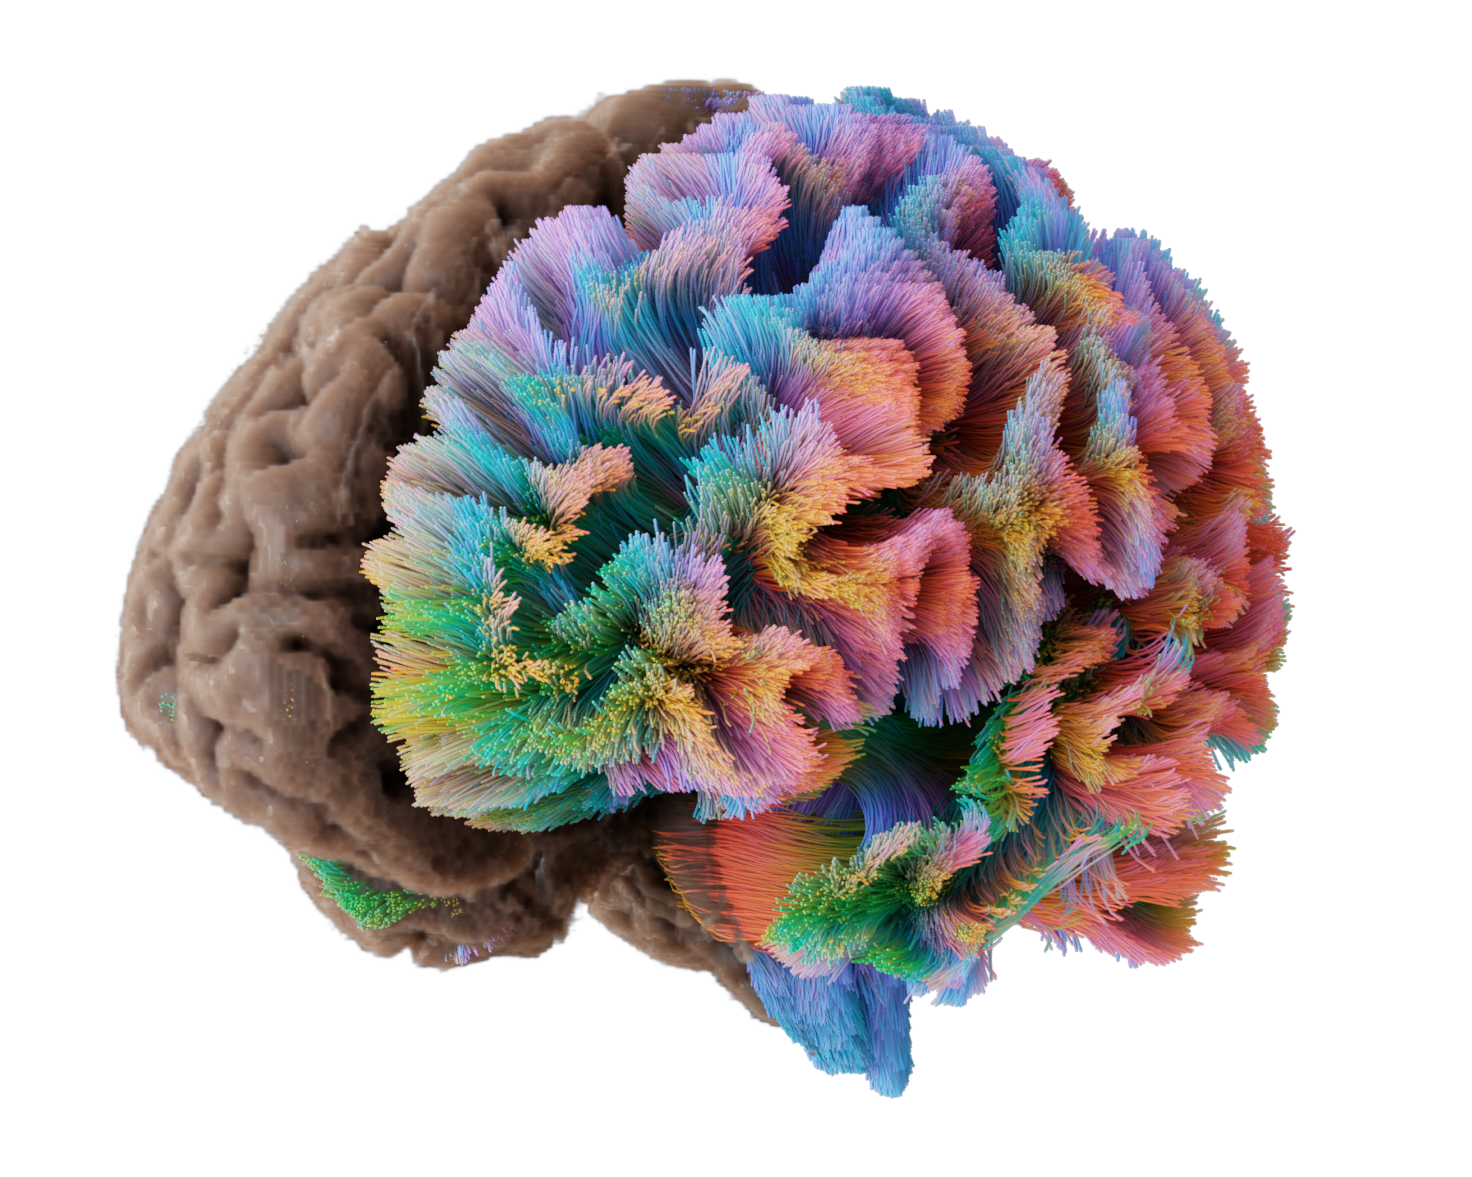
\includegraphics[width=\textwidth]{figures/hero.png}
        \caption{Whole-brain tractogram: Uniform thickness causes severe occlusion.}
        \label{fig:hero}
    \end{subfigure}
    \vspace{-0.2cm}
    \caption{Baseline tractography in Vibrant. All fibers share a single global radius parameter.}
    \label{fig:baseline}
\end{figure}

\vspace{-0.3cm}
\noindent \textbf{Our Proposed Solution:}
We adopt the \textbf{TRX format} \cite{trxformat} to load streamline geometry alongside per-vertex (\texttt{dpv}) and per-streamline (\texttt{dps}) scalars (e.g., Fractional Anisotropy, SIFT2 weights, length). We then use these attributes to feed:
\begin{enumerate}[leftmargin=*,nosep]
    \item \textbf{Varying Tube Thickness:} Ray-casting truncated cones with spherical end caps (Gro\ss{} \& Gumhold \cite{gross2021advanced}) so fibers taper organically at cortical tips and swell in dense bundles.
    \item \textbf{Varying Opacity:} Fading low-confidence fibers into semi-transparent lines to reveal core pathways.
    \item \textbf{Varying Color:} Colormapping scalars or direct RGB channels.
\end{enumerate}

\section{Requirements (MoSCoW)}
\begin{table}[ht!]
\centering
\small
\begin{tabularx}{\textwidth}{l p{4.6cm} X p{3.5cm}}
\toprule
\textbf{Priority} & \textbf{Feature} & \textbf{Technical Scope} & \textbf{Acceptance Criteria} \\
\midrule
\textbf{Must-Have} & \textbf{M1: TRX Ingestion (\texttt{trx-rs})} & Load \texttt{.trx} files (geometry + \texttt{dpv}/\texttt{dps} tables) into a unified Tractogram model (keeping \texttt{.tck}/\texttt{.tsf} support). & Loads official reference bundles (AF, CST) and extracts attributes. \\
\textbf{Must-Have} & \textbf{M2: Rounded Cones (WGSL)} & Ray-cast truncated cones with spherical end caps ($P_A, r_A \to P_B, r_B$) with tilted analytical normals. & Smooth joints without cracks; correct highlights under PBR lighting. \\
\textbf{Must-Have} & \textbf{M3: Radius-Aware Voxel Grid} & Update \texttt{voxelize.wgsl} to bound segments by $r_{\max} = \max(r_A, r_B)$ in the voxel acceleration structure. & Zero ray-leak holes during interactive 3D rotation at 100k lines. \\
\textbf{Must-Have} & \textbf{M4: Interactive Mapping UI} & \texttt{egui} sliders mapping scalar attributes to physical radius $[r_{\min}, r_{\max}]$ in mm. & Real-time update ($< 16\,\text{ms}$) on slider change without geometry re-upload. \\
\midrule
\textbf{Should-Have} & \textbf{S1: Varying Opacity} & Map confidence scalars to stochastic transparency/thresholding. & Low-confidence fibers fade smoothly; interactive de-cluttering. \\
\textbf{Should-Have} & \textbf{S2: Varying Color} & Route scalar attributes through custom colormaps or RGB data. & Multi-attribute visual distinction. \\
\textbf{Should-Have} & \textbf{S3: Tip Tapering} & Procedural tapering of endpoints toward zero radius at cortex. & Natural anatomical bundle terminations. \\
\midrule
\textbf{Could-Have} & \textbf{C1: 3D Volume Sampling} & Compute pass sampling 3D NIfTI volumes at vertices live. & Fibers dynamically adapt color/radius near tumor/lesion masks. \\
\bottomrule
\end{tabularx}
\caption{Prioritized project requirements with concrete acceptance criteria.}
\end{table}

\section{Technical Architecture}

\noindent \textbf{Pipeline:} The data flows from files into a unified model, which feeds GPU buffers and shaders:
\begin{center}
\small
\begin{tcolorbox}[colback=white,colframe=bordergray]
\centering
\texttt{.trx} (via \texttt{trx-rs}) \quad / \quad \texttt{.tck} + \texttt{.tsf}
$\quad\longrightarrow\quad$
\textbf{Unified Tractogram (Rust):} Positions, Offsets, \texttt{dpv}/\texttt{dps}\\
$\Big\downarrow$ \emph{Interactive Mapping Layer (\texttt{egui}): Radius $[r_{\min}, r_{\max}]$, Opacity $\alpha$, Color}\\
\textbf{GPU Buffer Streaming:} Packed Vertex Buffer $(\mathbf{p}, r_v, \alpha_v)$\\
$\swarrow$ \hspace{5cm} $\searrow$\\
\textbf{Voxelization (\texttt{voxelize.wgsl}):} Slab $\max(r_A, r_B)$ \hspace{1cm} \textbf{Ray Tracing (\texttt{trace.wgsl}):} Rounded Cones
\end{tcolorbox}
\end{center}

\noindent \textbf{Rounded Cone Math:} For a segment connecting $P_A(r_A)$ to $P_B(r_B)$ with length $L = \|P_B - P_A\|$, the cone opening half-angle is $\sin \alpha = (r_A - r_B)/L$. The ray intersection solves the cone quadratic $at^2 + 2bt + c = 0$ bounded between tangent circles, plus the two spherical end caps. The surface normal is tilted by $\alpha$ along the segment axis. When $|r_A - r_B| < 10^{-4}$, the shader executes the fast cylinder fallback.

\section{Team Roles and 8-Week Timeline}
The workload is split equitably ($33.3\%$ each) across three non-overlapping layers:
\begin{itemize}[leftmargin=*,nosep]
    \item \textbf{Student 1 (Graphics / Shaders):} WGSL rounded cone ray intersection (\texttt{intersect.wgsl}), analytical surface normals, and radius-aware voxelization (\texttt{voxelize.wgsl}).
    \item \textbf{Student 2 (Systems / Engine):} \texttt{trx-rs} integration in \texttt{src/file/line.rs}, in-memory Tractogram data structures, and GPU vertex buffer packing.
    \item \textbf{Student 3 (UI / Interaction / QA):} \texttt{egui} transfer panel (radius/opacity sliders), synthetic test suite (helix with varying $r$), and 60+ FPS benchmarking.
\end{itemize}

\begin{table}[ht!]
\centering
\small
\begin{tabularx}{\textwidth}{c l p{7.5cm} X}
\toprule
\textbf{Week} & \textbf{Phase} & \textbf{Milestone Objectives} & \textbf{Deliverable} \\
\midrule
\textbf{W1--W2} & Setup \& Scoping & Environment setup, math derivation, scoping document. & Approved scoping document. \\
\textbf{W3--W4} & Core Shaders \& TRX & Implement \texttt{cone\_intersection}; integrate \texttt{trx-rs} archive loader. & Crack-free cone render on test helix. \\
\textbf{W5} & Voxel Acceleration & Update \texttt{voxelize.wgsl} for $\max(r_A, r_B)$; pack GPU attribute buffer. & Zero ray-leak holes during rotation. \\
\textbf{W6} & UI \& Opacity & \texttt{egui} radius/opacity mapping panel; stochastic alpha modulation. & Real-time interactive attribute scaling. \\
\textbf{W7} & Color \& Polish & Multi-channel colormapping, cortical endpoint tapering. & Polished rendering across all bundles. \\
\textbf{W8} & Evaluation & Performance benchmarking ($\ge 60\,\text{FPS}$), final presentation \& report. & Final code PR and report. \\
\bottomrule
\end{tabularx}
\caption{8-week project milestone schedule.}
\end{table}

\vspace{-0.3cm}
\bibliographystyle{plain}
\bibliography{references}

\end{document}
